\documentclass[border=10pt]{standalone}
\usepackage{tikz}
\usetikzlibrary{arrows.meta, calc, decorations.pathreplacing}

\begin{document}

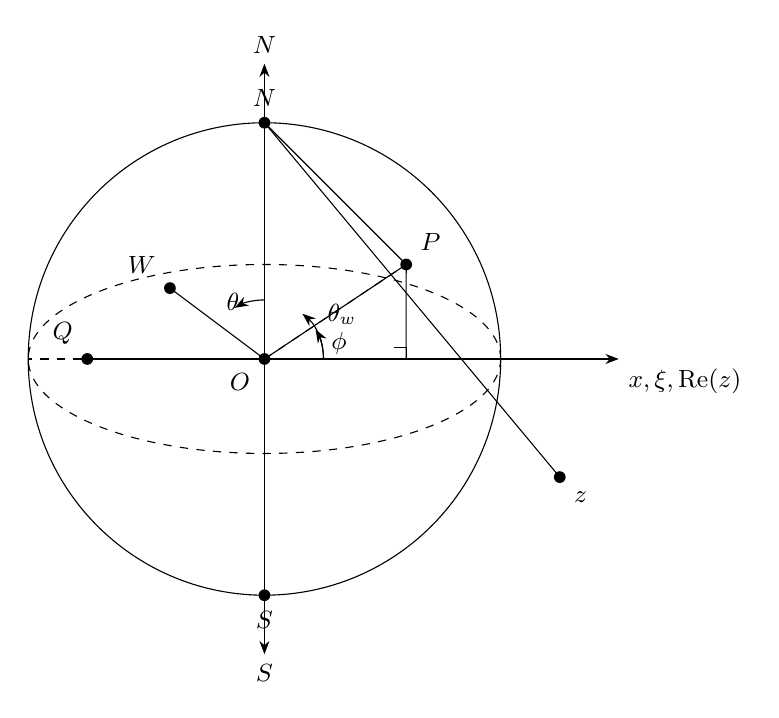
\begin{tikzpicture}[
    scale=1.5,
    >=Stealth,
    every node/.style={font=\small},
    point/.style={circle, fill, inner sep=1.5pt}
]

% Define key points
\coordinate (O) at (0,0);
\coordinate (N) at (0,2);
\coordinate (S) at (0,-2);
\coordinate (P) at (1.2,0.8);
\coordinate (Q) at (-1.5,0);
\coordinate (W) at (-0.8,0.6);
\coordinate (z) at (2.5,-1);

% Draw sphere (circle)
\draw (O) circle (2);

% Draw equator (dashed)
\draw[dashed] (O) ellipse (2 and 0.8);

% Draw meridian (dashed)
\draw[dashed] (N) -- (S);

% Draw axes
\draw[->] (O) -- (3,0) node[below right] {$x, \xi, \mathrm{Re}(z)$};
\draw[->] (O) -- (0,2.5) node[above] {$N$};
\draw[->] (O) -- (0,-2.5) node[below] {$S$};

% Draw points
\node[point, label=above right:$P$] at (P) {};
\node[point, label=above left:$W$] at (W) {};
\node[point, label=above left:$Q$] at (Q) {};
\node[point, label=below right:$z$] at (z) {};
\node[point, label=above:$N$] at (N) {};
\node[point, label=below:$S$] at (S) {};
\node[point, label=below left:$O$] at (O) {};

% Draw lines
\draw (O) -- (P);
\draw (O) -- (Q);
\draw (O) -- (W);
\draw (N) -- (P);
\draw (N) -- (z);
\draw (P) -- (1.2,0) coordinate (Pproj); % projection to equator
\draw (O) -- (Pproj);

% Right angle mark
\draw (1.2,0) -- ++(0,0.1) -- ++(-0.1,0);

% Angles
\draw[->] (0.5,0) arc (0:30:0.5) node[midway, right] {$\phi$};
\draw[->] (0.5,0) arc (0:50:0.5) node[midway, above right] {$\theta_w$};
\draw[->] (0,0.5) arc (90:120:0.5) node[midway, left] {$\theta$};

% Dashed lines for perspective
\draw[dashed] (O) -- (-2,0);
\draw[dashed] (O) -- (0,0.8);
\draw[dashed] (O) -- (1.2,0.8);

\end{tikzpicture}

\end{document}